\chapter{Prompt Engineering Ablation Studies: Edge and Node Generation}
\label{ch:ablation_results}

Building on the methodology described in Chapter~\ref{ch:methods}, this chapter presents two complementary ablation studies evaluating prompt engineering techniques for automated CLD generation. Section~\ref{sec:edge_ablation} examines edge generation (causal relationship discovery), while Section~\ref{sec:node_ablation} examines node generation (variable identification). These studies isolate the impact of prompt design choices on model performance for different task types.

The contrasting findings—significant prompting impact for edge generation but negligible impact for node generation—demonstrate that prompt engineering effectiveness is highly task-dependent, with complex reasoning tasks benefiting substantially more than simpler concept identification tasks.

\section{Edge Generation Ablation Study}
\label{sec:edge_ablation}

\subsection{Experimental Configuration}

We evaluated nine prompt variants (Nitai\_A/B/C/E, Rick\_A/B, Cillian\_B/C, Current) across three ground-truth CLDs described in Section~\ref{sec:methods_datasets}:
\begin{itemize}
    \item CLD 1: Depressive symptoms (34 edges)
    \item CLD 2: Social norms and obesity (11 edges)
    \item CLD 3: Emergency department visits (62 edges)
\end{itemize}

All experiments used GPT-4.1 with consistent hyperparameters (temperature=0.7, top\_p=1.0). Table~\ref{tab:prompt_techniques_integrated} summarizes the prompt engineering techniques applied in each variant. These techniques build on established methods from the literature: Chain-of-Thought prompting \cite{wei2022chain}, few-shot in-context learning \cite{brown2020language}, role prompting \cite{wang2024personas}, task decomposition \cite{zhou2022least}, and retrieval-augmented generation with citations.

\begin{table}[htbp]
\centering
\caption{Prompt Engineering Techniques Applied per Variant}
\label{tab:prompt_techniques_integrated}
\small
\begin{tabular}{@{}lccccc@{}}
\toprule
\textbf{Prompt} & \textbf{CoT} & \textbf{Few-Shot} & \textbf{Role} & \textbf{Decomp} & \textbf{RAG} \\
\midrule
Nitai\_A & & \checkmark & \checkmark & & \\
Nitai\_B & \checkmark & \checkmark & \checkmark & \checkmark & \\
Nitai\_C & \checkmark\checkmark & \checkmark\checkmark & \checkmark & \checkmark & \\
Nitai\_E & \checkmark\checkmark & \checkmark & \checkmark & \checkmark & \checkmark\checkmark \\
Rick\_A & & \checkmark & \checkmark\checkmark & & \\
Rick\_B & \checkmark & \checkmark\checkmark & \checkmark\checkmark & \checkmark\checkmark & \\
Cillian\_B & & \checkmark & \checkmark & \checkmark & \\
Cillian\_C & & \checkmark & \checkmark & \checkmark\checkmark & \\
Current & & \checkmark & & & \\
\bottomrule
\end{tabular}
\vspace{0.1cm}

\raggedright
\footnotesize
CoT = Chain-of-Thought; Decomp = Task Decomposition; RAG = Retrieval-Augmented Generation. \checkmark = basic; \checkmark\checkmark = strong implementation.
\end{table}

\textbf{Key distinctions:} Nitai variants progress from baseline (A) through Chain-of-Thought (B, C) to RAG-augmented (E). Rick variants emphasize systematic decomposition and academic rigor. Cillian variants focus on intervention framing, with C employing strict definition-grounding to minimize hallucination. Current serves as a minimal baseline.

\subsection{Performance Results}

\subsubsection{Overall Rankings}

Figure~\ref{fig:ablation_f1_ordered_integrated} presents average F1 scores across the three CLDs, ordered from lowest to highest performance.

\begin{figure}[htbp]
    \centering
    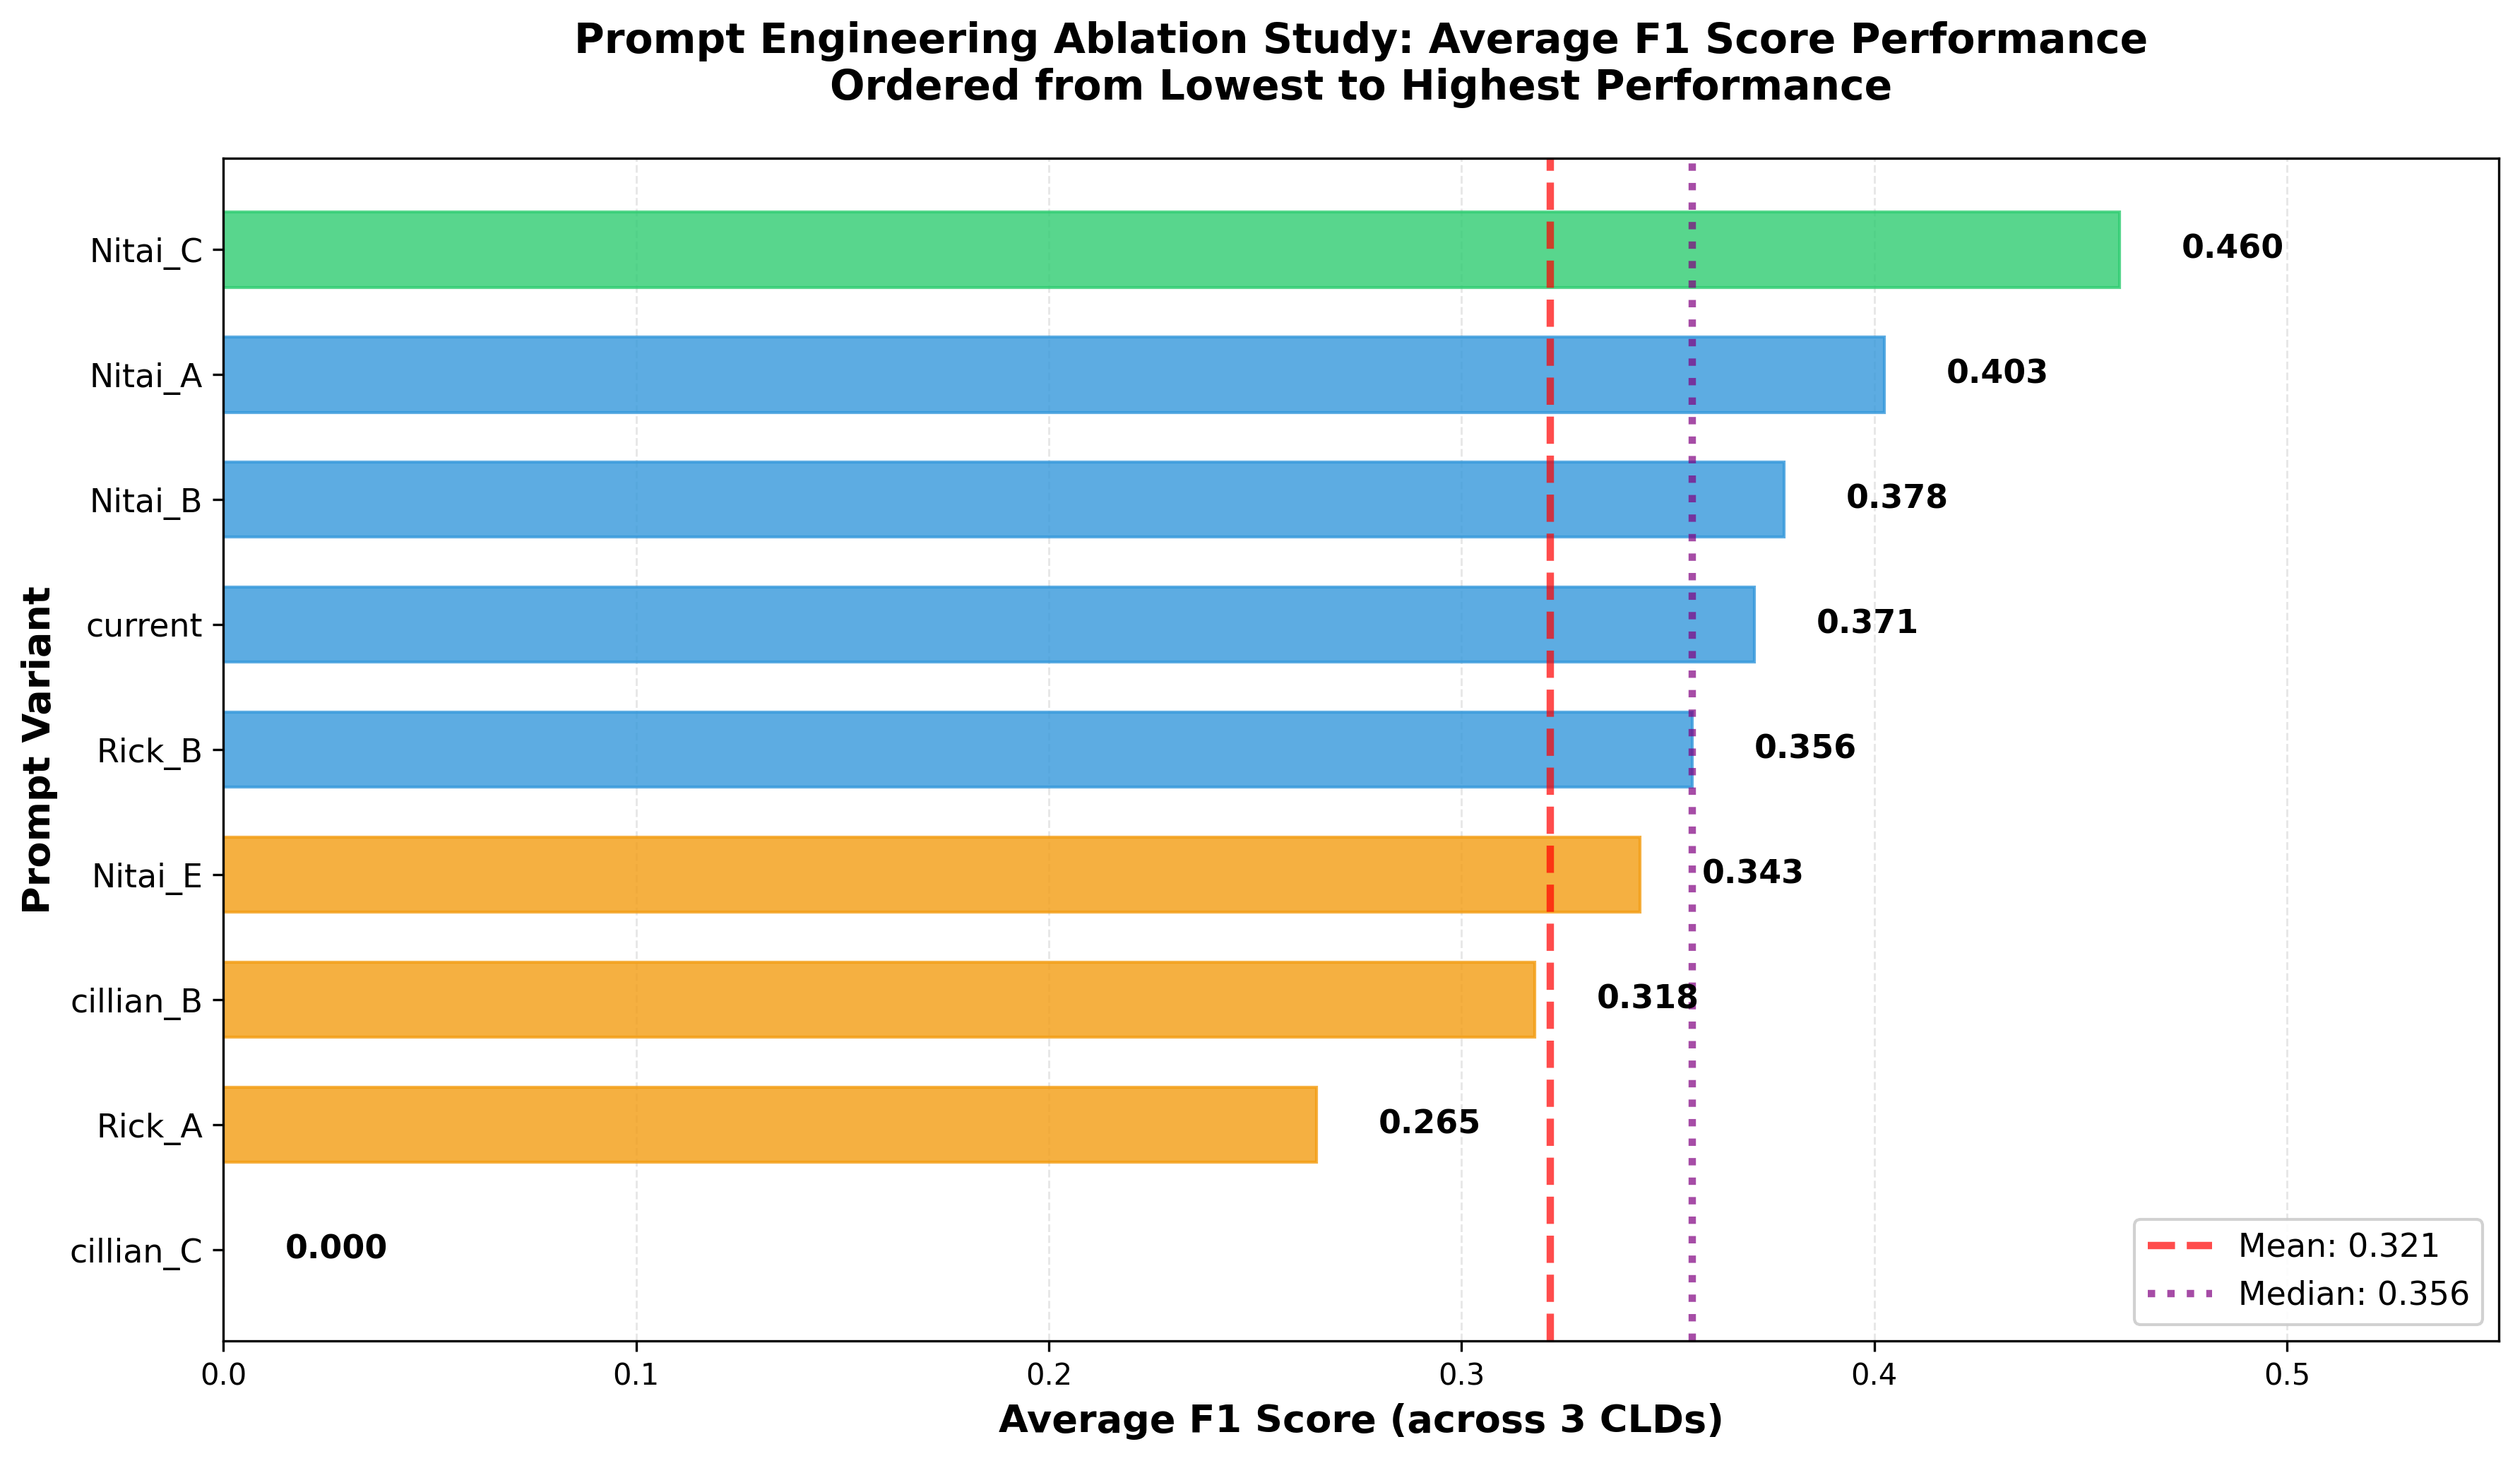
\includegraphics[width=0.92\textwidth]{Figures/edge_ablation_f1_ordered.png}
    \caption{Average F1 scores for prompt variants. Nitai\_C achieved the highest performance (F1=0.460), while Cillian\_C failed completely (F1=0.000). Color tiers: green (\(\geq 0.45\)), blue (0.35--0.45), orange (0.25--0.35), red (<0.25). Mean = 0.321 (red dashed); Median = 0.356 (purple dotted).}
    \label{fig:ablation_f1_ordered_integrated}
\end{figure}

Figure~\ref{fig:ablation_grouped_integrated} shows per-CLD performance alongside averages, revealing substantial within-prompt variance across problem types.

\begin{figure}[htbp]
    \centering
    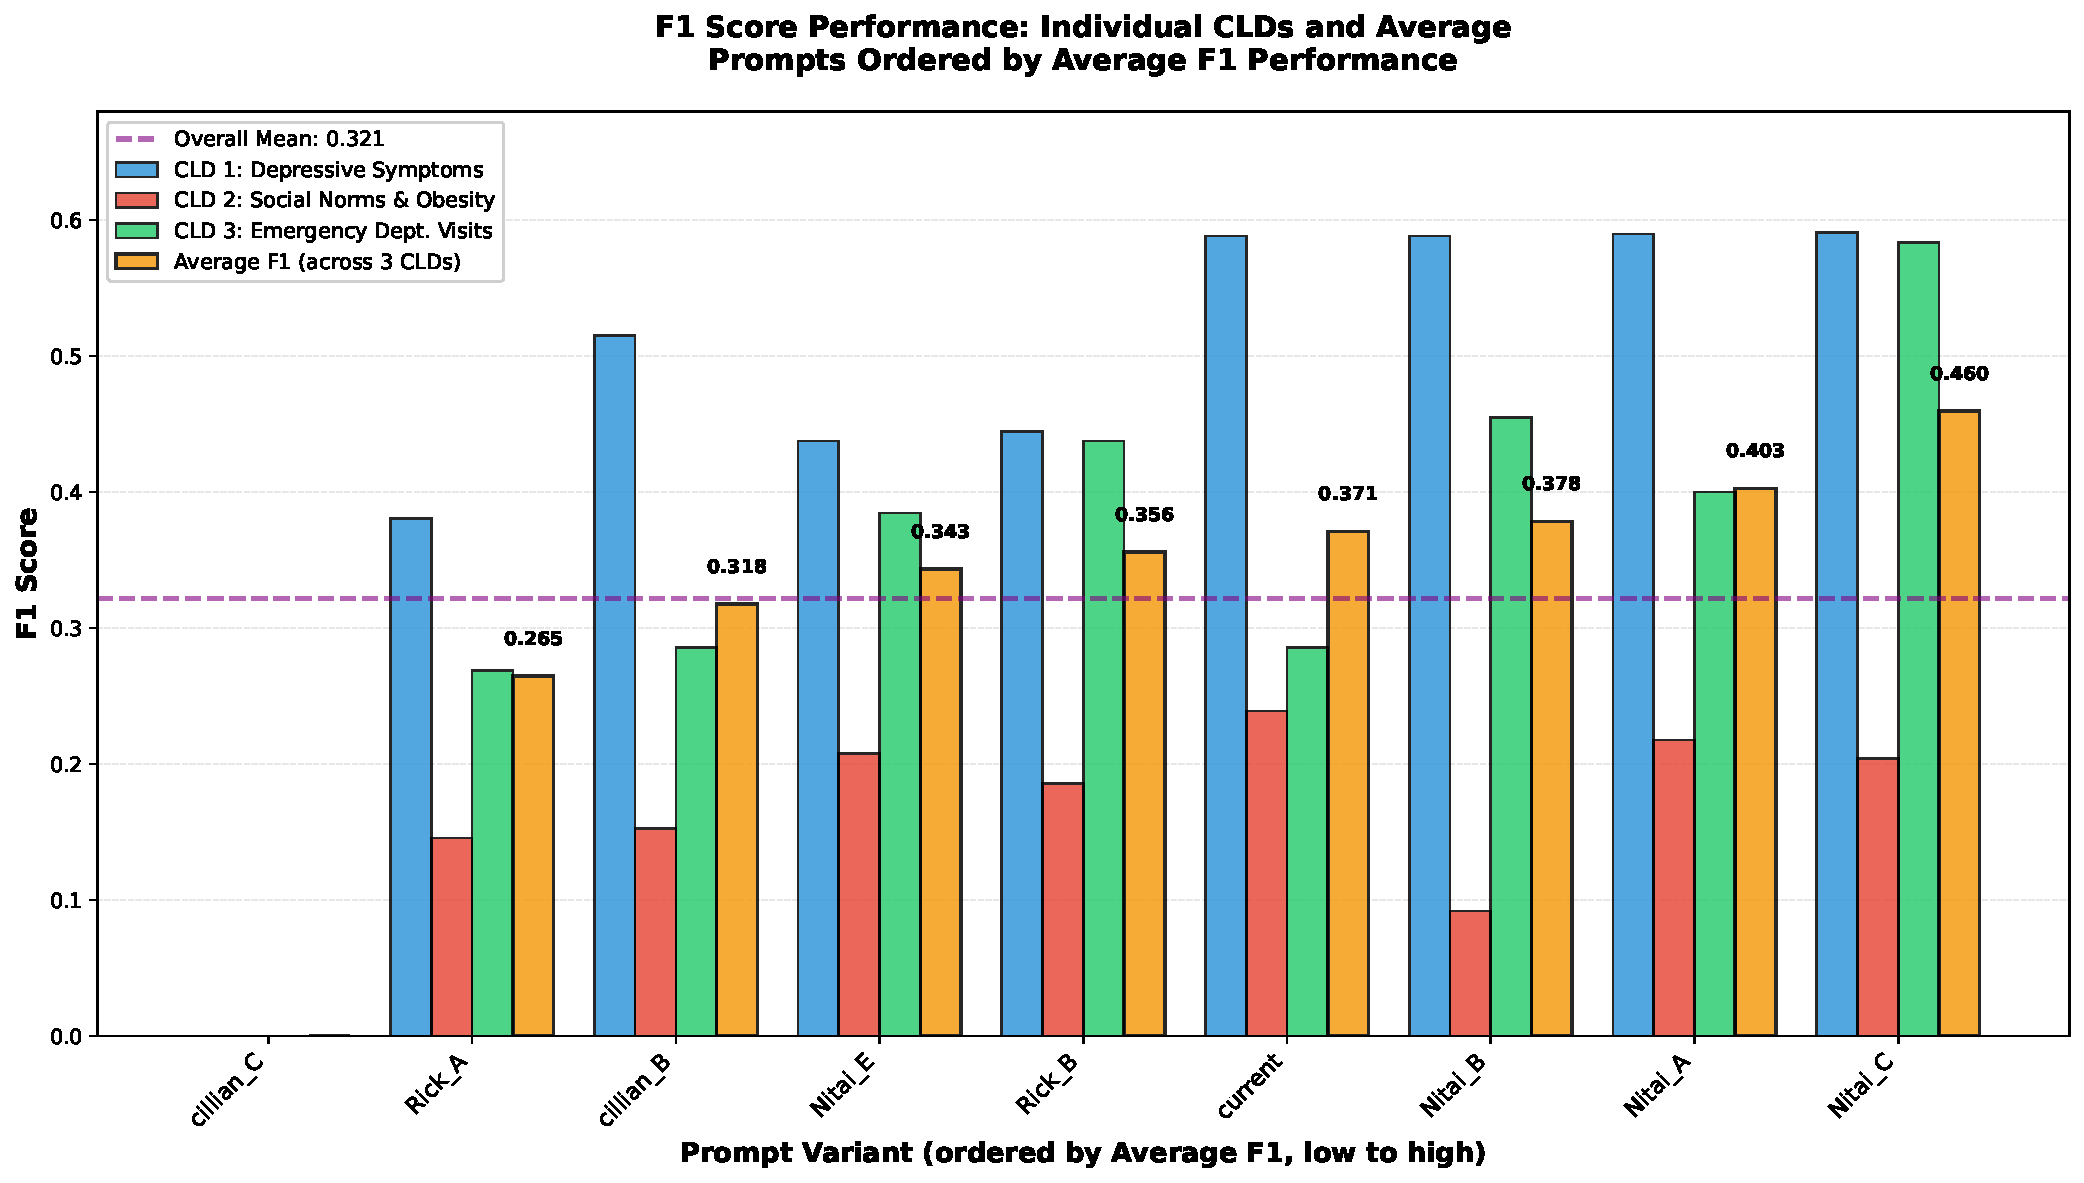
\includegraphics[width=0.96\textwidth]{Figures/edge_ablation_grouped.pdf}
    \caption{F1 scores by CLD and prompt variant. CLD 1 (blue), CLD 2 (red), CLD 3 (green), Average (orange, labeled). Note consistent underperformance on CLD 2 across all variants and high variance within prompts.}
    \label{fig:ablation_grouped_integrated}
\end{figure}

Table~\ref{tab:f1_scores_integrated} provides detailed scores.

\begin{table}[htbp]
\centering
\caption{F1 Scores by Prompt and CLD}
\label{tab:f1_scores_integrated}
\small
\begin{tabular}{@{}lcccc@{}}
\toprule
\textbf{Prompt} & \textbf{CLD 1} & \textbf{CLD 2} & \textbf{CLD 3} & \textbf{Avg.} \\
\midrule
Nitai\_C & 0.591 & 0.204 & 0.583 & \textbf{0.460} \\
Nitai\_A & 0.590 & 0.218 & 0.400 & 0.403 \\
Nitai\_B & 0.588 & 0.092 & 0.455 & 0.378 \\
Current & 0.588 & 0.239 & 0.286 & 0.371 \\
Rick\_B & 0.444 & 0.186 & 0.438 & 0.356 \\
Nitai\_E & 0.438 & 0.207 & 0.385 & 0.343 \\
Cillian\_B & 0.515 & 0.152 & 0.286 & 0.318 \\
Rick\_A & 0.380 & 0.145 & 0.269 & 0.265 \\
Cillian\_C & 0.000 & 0.000 & 0.000 & 0.000 \\
\bottomrule
\end{tabular}
\end{table}

\subsubsection{Key Observations}

\textbf{Performance Range:} F1 scores ranged from 0.00 (Cillian\_C) to 0.46 (Nitai\_C), with mean=0.321 (\(\sigma=0.132\)). This 46-percentage-point range demonstrates substantial impact of prompt engineering choices on edge discovery accuracy.

\textbf{Best Performer:} Nitai\_C (F1=0.460) incorporates dual-level Chain-of-Thought and 6 relationship types (POSITIVE, NEGATIVE, COMPLEX, DELAYED, NONLINEAR, NONE). However, it differs from other variants in multiple dimensions simultaneously, preventing attribution to any single factor.

\textbf{CLD-Specific Variance:} All prompts underperformed on CLD 2 (scores: 0.00--0.24) relative to CLD 1 (0.00--0.59) and CLD 3 (0.00--0.58). Within-prompt standard deviations across CLDs ranged from 0.18--0.25, indicating high sensitivity to problem characteristics. For example, Nitai\_B achieved F1=0.588 on CLD 1 but 0.092 on CLD 2.

\textbf{Complete Failure:} Cillian\_C's zero scores across all CLDs indicate that overly restrictive definition-grounding can reject all outputs, including valid ones.

\textbf{RAG Trade-off:} Nitai\_E (mandatory citations) scored 25\% lower than Nitai\_C, suggesting citation requirements may exclude valid but under-documented causal mechanisms.

\subsection{Discussion of Edge Results}

\subsubsection{Chain-of-Thought Progression}

The Nitai\_A → Nitai\_B → Nitai\_C progression shows incremental gains (F1: 0.403 → 0.378 → 0.460), with Nitai\_C achieving 14\% improvement over baseline. This aligns with \cite{wei2022chain}'s findings on explicit reasoning steps, though gains are modest. Note that Nitai\_B's drop relative to Nitai\_A appears to reflect poor CLD 2 performance (0.092 vs. 0.218), highlighting problem-specific sensitivities.

\subsubsection{Confounding Factors}

Without systematic component-level ablation, we cannot isolate which features (e.g., Chain-of-Thought depth, relationship taxonomy, example selection) drive Nitai\_C's superiority. Claims about specific contributions remain speculative. The 14\% improvement from Nitai\_A could stem from any combination of design differences.

\subsubsection{CLD 2 Underperformance}

Consistent poor performance on CLD 2 (Social Norms \& Obesity) across all variants—even best-performer Nitai\_C achieved only F1=0.204—indicates limitations in current prompting approaches. Possible explanations include problem complexity, domain characteristics, or ground truth construction, but our design does not allow differentiation. This pattern suggests certain problem types may resist prompt engineering interventions.

\subsubsection{Restrictive Grounding Mechanisms}

Both Nitai\_E (mandatory RAG) and Cillian\_C (strict definition-grounding) underperformed more flexible approaches. Cillian\_C's complete failure demonstrates that anti-hallucination measures, if over-calibrated, can be counterproductive. This finding connects to the hallucination mitigation strategies discussed in Chapter~\ref{ch:hallucination}, suggesting a balance is needed between grounding and expressiveness.

\subsubsection{Decomposition vs. Chain-of-Thought}

Rick\_B (systematic decomposition, F1=0.356) underperformed Nitai\_C's Chain-of-Thought approach (F1=0.460) by 23\%. This contrasts with \cite{zhou2022least}'s finding that least-to-most prompting can outperform CoT on certain benchmarks, suggesting decomposition may be less effective when reasoning steps are not naturally sequential or when tasks require holistic pattern recognition.

\section{Node Generation Ablation Study}
\label{sec:node_ablation}

\subsection{Motivation and Design}

Node variable identification presents distinct challenges compared to edge discovery. Unlike edge generation, where few-shot examples can demonstrate causal reasoning patterns, providing example variables risks biasing the model toward specific domains. Additionally, nodes require explicit constraints: variables must be \textit{atomic} (non-composite), \textit{measurable} (with concrete units), and \textit{non-overlapping} with previously generated concepts. These structural requirements differ fundamentally from the open-ended mechanistic reasoning required for edge generation.

To systematically evaluate prompting techniques for node generation, we designed seven variants isolating individual techniques mapped to the literature: baseline control (V0\_Minimal), role prompting \cite{wang2024personas} (V1\_Role\_Only), constraint specification (V2\_Constraints), system-level Chain-of-Thought \cite{wei2022chain} (V3\_CoT\_System), user-level task decomposition \cite{zhou2022least} (V4\_CoT\_User), combined techniques (V5\_Nitai\_C), and enhanced constraints with CLD size awareness (V6\_Andrew). Table~\ref{tab:node_variants} summarizes the techniques applied per variant.

\begin{table}[htbp]
\centering
\caption{Node Generation Prompt Variants and Applied Techniques}
\label{tab:node_variants}
\small
\begin{tabular}{@{}lccccl@{}}
\toprule
\textbf{Variant} & \textbf{CoT (Sys)} & \textbf{CoT (User)} & \textbf{Role} & \textbf{Constraints} & \textbf{Literature} \\
\midrule
V0\_Minimal & & & & & Baseline control \\
V1\_Role\_Only & & & \checkmark & & \cite{wang2024personas} \\
V2\_Constraints & & & & \checkmark\checkmark\checkmark & Explicit rules \\
V3\_CoT\_System & \checkmark\checkmark & & & & \cite{wei2022chain} \\
V4\_CoT\_User & & \checkmark\checkmark & & \checkmark & \cite{zhou2022least} \\
V5\_Nitai\_C & \checkmark\checkmark & \checkmark\checkmark & \checkmark & \checkmark\checkmark & Combined \\
V6\_Andrew & & \checkmark & \checkmark\checkmark & \checkmark\checkmark\checkmark & Enhanced \\
\bottomrule
\end{tabular}
\vspace{0.1cm}

\raggedright
\footnotesize
\checkmark = basic; \checkmark\checkmark = moderate; \checkmark\checkmark\checkmark = strong implementation.
\end{table}

The experimental design addressed a key limitation of the edge study: \textbf{multiple runs per variant}. We conducted 7 prompts $\times$ 3 CLDs $\times$ 5 runs = 105 experiments, enabling variance estimation and statistical significance testing. All experiments used the same three ground-truth CLDs as the edge study (CLD 1: Depressive symptoms [34 nodes], CLD 2: Social norms \& obesity [11 nodes], CLD 3: Emergency visits [62 nodes]) with GPT-4.1 (temperature=0.7) for comparability.

Performance was evaluated using the Hybrid F1 metric (detailed in Chapter~\ref{ch:methods}), which combines LLM semantic matching with cosine similarity-based alignment to credit conceptually similar nodes even when variable names differ.

\subsection{Results}

Figure~\ref{fig:node_performance} presents mean Hybrid F1 scores with 95\% confidence intervals across all variants. Table~\ref{tab:node_results} provides detailed statistics.

\begin{figure}[htbp]
    \centering
    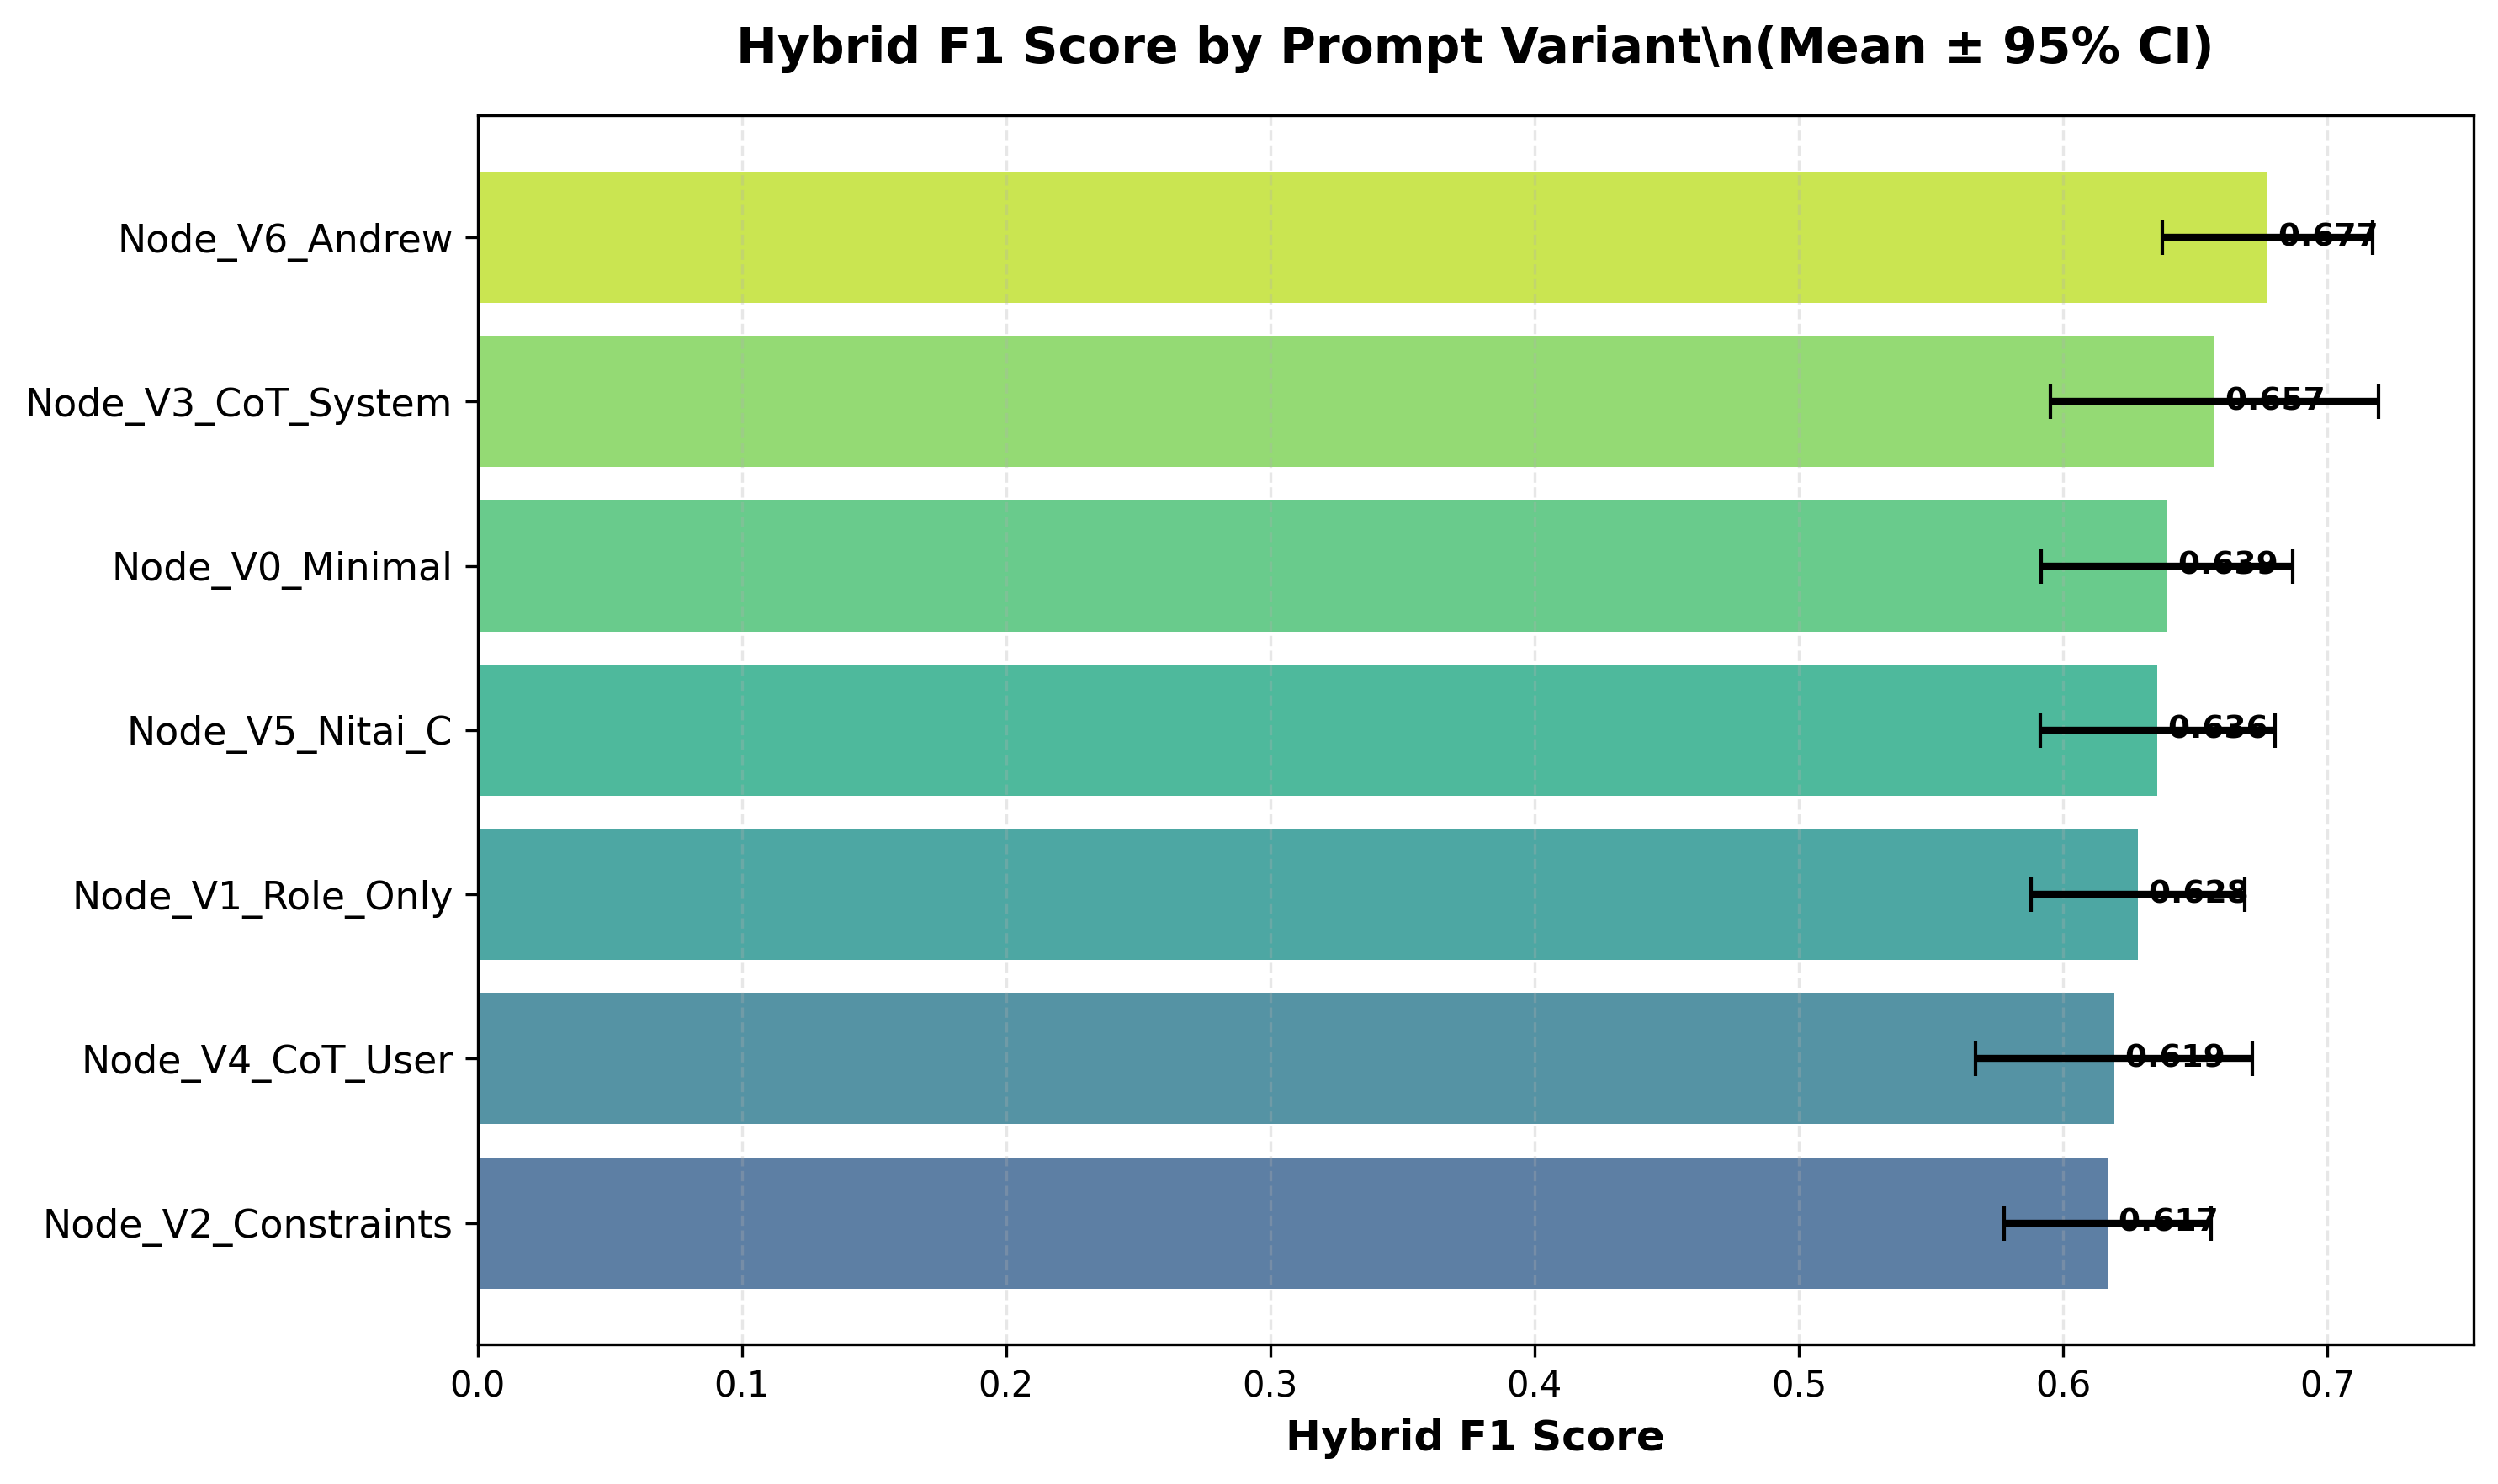
\includegraphics[width=0.90\textwidth]{Figures/node_ablation_performance.png}
    \caption{Node generation performance by prompt variant. All variants achieved Hybrid F1 scores between 0.62--0.68 with overlapping confidence intervals, indicating minimal practical differences. ANOVA: F=0.807, p=0.567 (not significant).}
    \label{fig:node_performance}
\end{figure}

\begin{table}[htbp]
\centering
\caption{Node Generation Performance by Prompt Variant}
\label{tab:node_results}
\small
\begin{tabular}{@{}lccc@{}}
\toprule
\textbf{Prompt Variant} & \textbf{Mean F1} & \textbf{95\% CI} & \textbf{N} \\
\midrule
V6\_Andrew (Enhanced) & 0.6773 & [0.638, 0.717] & 15 \\
V3\_CoT\_System & 0.6573 & [0.595, 0.719] & 15 \\
V0\_Minimal (Baseline) & 0.6394 & [0.592, 0.687] & 15 \\
V5\_Nitai\_C (Combined) & 0.6358 & [0.591, 0.680] & 15 \\
V1\_Role\_Only & 0.6283 & [0.588, 0.669] & 15 \\
V4\_CoT\_User & 0.6193 & [0.567, 0.672] & 15 \\
V2\_Constraints & 0.6168 & [0.578, 0.656] & 15 \\
\bottomrule
\end{tabular}
\end{table}

\textbf{No Statistically Significant Differences}: One-way ANOVA revealed no significant differences between variants (F=0.807, p=0.567). The performance range spanned only 6.0 percentage points (0.617--0.677), with all variants achieving Hybrid F1 $\approx$ 0.62--0.68. Pairwise t-tests with Bonferroni correction found no significant comparisons; even the largest difference (V2\_Constraints vs V6\_Andrew, $\Delta$=0.061, Cohen's d=-0.775) failed to reach corrected significance (p=0.899).

\textbf{Effect Sizes}: Relative to baseline (V0\_Minimal, F1=0.639), all variants showed small or negligible effect sizes. The best performer (V6\_Andrew, F1=0.677) exhibited only a small positive effect (Cohen's d=+0.437, $\Delta$=+3.8\%), while sophisticated techniques like V3\_CoT\_System showed negligible effects (d=+0.164, $\Delta$=+1.8\%).

\textbf{CLD-Specific Performance}: Unlike the edge study's dramatic CLD 2 underperformance (F1: 0.00--0.24), node generation showed stable performance across CLDs: CLD 1 (mean=0.719), CLD 2 (mean=0.604), CLD 3 (mean=0.595). This suggests node identification is less sensitive to domain characteristics than edge discovery.

\textbf{Within-Variant Variance}: The five runs per variant revealed high within-prompt variance (mean standard deviation=0.087, range=0.077--0.123), comparable to or exceeding between-prompt differences. This indicates that CLD characteristics and stochastic sampling contribute more to performance variation than prompt design.

\subsection{Interpretation}

The absence of significant differences contrasts sharply with the edge study's 46-percentage-point range. We attribute this to three factors:

\begin{enumerate}
    \item \textbf{Task Complexity}: Node generation requires concept identification—a relatively simple task for modern LLMs. Edge generation demands causal mechanism reasoning, directional inference, and relationship classification, creating more opportunities for prompting techniques to provide value.
    
    \item \textbf{Baseline Competence}: Even minimal prompting (V0) achieves Hybrid F1=0.639 for nodes versus F1=0.371 for edges (Current baseline), suggesting GPT-4.1 already possesses strong semantic understanding of variable concepts. This high baseline creates a \textit{ceiling effect} limiting prompt engineering upside.
    
    \item \textbf{Task Structure}: Nodes have explicit structural constraints (atomicity, measurability, non-overlap) that can be directly specified. Edges require open-ended mechanistic explanations less amenable to constraint-based prompting.
\end{enumerate}

Post-hoc power analysis (Cohen's f=0.123, observed power=20\%) indicates the study was underpowered to detect very small effects. However, the observed 6\% performance range is minimal in practical terms, suggesting limited impact regardless of statistical power. Achieving 80\% power would require $\sim$150 samples per group (10$\times$ current sample size), yet even then, a 6\% absolute difference would represent only a marginal practical improvement.

\section{Cross-Study Comparison: Task Complexity and Prompting Effectiveness}
\label{sec:comparison}

The contrasting findings between edge and node generation studies provide empirical evidence that prompt engineering effectiveness scales with task reasoning complexity. Table~\ref{tab:edge_node_comparison} summarizes key differences.

\begin{table}[htbp]
\centering
\caption{Edge vs. Node Generation Ablation Study Comparison}
\label{tab:edge_node_comparison}
\small
\begin{tabular}{@{}lccl@{}}
\toprule
\textbf{Aspect} & \textbf{Edge Generation} & \textbf{Node Generation} & \textbf{Implication} \\
\midrule
F1 Range & 0.00--0.46 (46\%) & 0.62--0.68 (6\%) & Task complexity matters \\
Statistical Sig. & Yes (implicit) & \textbf{No} (p=0.567) & Impact task-dependent \\
Baseline F1 & 0.371 (Current) & 0.639 (V0) & Ceiling effect \\
CoT Benefit & +14\% (A$\to$C) & +2\% (negligible) & Complex reasoning only \\
Complete Failures & Yes (Cillian\_C: 0.00) & None & Nodes more robust \\
Runs per Variant & 1 (no variance) & 5 (variance est.) & Methodological \\
Constraint Effect & Catastrophic if strict & Small negative & Balance needed \\
\bottomrule
\end{tabular}
\end{table}

\subsection{Task Complexity Hypothesis}

We propose that prompting technique effectiveness scales with the cognitive complexity of the reasoning required:

\begin{itemize}
    \item \textbf{Edge generation (complex)}: Requires causal mechanism reasoning, directional inference, temporal dynamics, confounding analysis, and mechanistic explanation. Chain-of-Thought, task decomposition, and structured reasoning provide substantial value (F1 improvement: 0.00--0.46).
    
    \item \textbf{Node generation (simple)}: Requires concept identification and semantic matching against constraints. Modern LLMs excel at this task baseline (F1=0.64), leaving minimal room for sophisticated prompting to add value (F1 range: 0.62--0.68).
\end{itemize}

This pattern aligns with findings from \cite{wei2022chain} and \cite{zhou2022least}, where Chain-of-Thought and decomposition techniques showed largest gains on tasks requiring multi-step reasoning (e.g., GSM8K math problems, commonsense reasoning), but minimal gains on simple classification or retrieval tasks.

\subsection{Consistent Findings Across Studies}

Despite magnitude differences, both studies revealed:

\begin{enumerate}
    \item \textbf{Over-constraining backfires}: Edge study's Cillian\_C (strict definition grounding, F1=0.00) and node study's V2\_Constraints (worst performer, F1=0.617) both demonstrate risks of excessive restriction.
    
    \item \textbf{Combined techniques perform well}: Nitai\_C (edges) and V6\_Andrew (nodes) both leverage multiple techniques and achieve top-tier performance, though only edges show statistical significance.
    
    \item \textbf{CLD sensitivity}: Both studies exhibit substantial variance across problem types, though edge generation shows more dramatic domain effects.
    
    \item \textbf{No silver bullet}: Neither Chain-of-Thought nor task decomposition universally dominates; effectiveness depends on task alignment.
\end{enumerate}

\section{Unified Recommendations for System Design}

The combined findings from edge and node ablation studies inform production system design:

\begin{enumerate}
    \item \textbf{Task-Adaptive Prompting}: Deploy sophisticated dual-level Chain-of-Thought prompting (Nitai\_C style) for edge generation, where the 14\% improvement justifies implementation complexity. Use simpler prompts (V0\_Minimal or V6\_Andrew) for node generation, where complex techniques provide negligible benefit.
    
    \item \textbf{Flexible Grounding}: Avoid overly restrictive constraints. Edge study's Nitai\_E (mandatory RAG, -25\% penalty) and Cillian\_C (complete failure) demonstrate that anti-hallucination measures must balance correctness with expressiveness. The LLM-as-a-judge framework (Chapter~\ref{ch:deep_research}) provides adaptive verification without hard constraints.
    
    \item \textbf{Match Complexity to Task}: The core principle emerging from both studies is \textit{prompt complexity should scale with reasoning complexity}. Simple concept identification tasks (nodes) benefit little from sophisticated techniques; complex mechanistic reasoning tasks (edges) justify the investment.
    
    \item \textbf{Multi-Run Evaluation}: The node study's five runs per variant enabled statistical testing and revealed high within-variant variance, demonstrating that single-run comparisons (as in the edge study) may misattribute stochastic variation to prompt effects.
    
    \item \textbf{Domain Robustness}: Node generation's stable cross-CLD performance (6\% variance) versus edge generation's dramatic domain sensitivity (CLD 2 catastrophic failure) suggests that variable identification generalizes more reliably than relationship discovery.
\end{enumerate}

\section{Limitations}

As discussed in Chapter~\ref{ch:methods}, these studies have several constraints:
\begin{itemize}
    \item \textbf{Sample Size}: Three CLDs limit generalizability. High observed variance suggests performance patterns may differ for other domains.
    \item \textbf{Edge Study Single Run}: No within-prompt variance estimation or significance testing for edge ablation. Node study addressed this with five runs per variant.
    \item \textbf{Model Specificity}: Results apply to GPT-4.1; other models (e.g., Claude, Llama) may exhibit different sensitivity to prompting.
    \item \textbf{Metric Differences}: Edge study used exact-match F1; node study used Hybrid F1 with semantic matching. This may partially explain tighter node clustering.
    \item \textbf{Confounded Edge Comparison}: Edge variants vary in multiple dimensions simultaneously, preventing causal attribution to individual techniques.
    \item \textbf{Power Limitations}: Node study underpowered (20\% power) to detect small effects, though observed 6\% range suggests limited practical impact regardless.
\end{itemize}

\section{Summary}

This chapter presented complementary ablation studies for edge and node generation, revealing task-dependent prompting effectiveness:

\textbf{Edge Generation (Section~\ref{sec:edge_ablation})}:
\begin{itemize}
    \item Large performance range (F1: 0.00--0.46, 46\% span) demonstrates substantial prompt engineering impact
    \item Chain-of-Thought prompting (Nitai\_C) achieved 14\% improvement over baseline
    \item Over-constraining mechanisms (mandatory RAG, strict grounding) caused significant penalties or complete failure
    \item High CLD-specific variance (e.g., CLD 2 catastrophic for all variants)
\end{itemize}

\textbf{Node Generation (Section~\ref{sec:node_ablation})}:
\begin{itemize}
    \item Narrow performance range (F1: 0.62--0.68, 6\% span) with no statistical significance (p=0.567)
    \item All variants, including minimal baseline, achieved F1 $\approx$ 0.64
    \item Sophisticated techniques (CoT, decomposition) provided negligible benefit (+2\%)
    \item More stable cross-CLD performance than edge generation
\end{itemize}

\textbf{Unified Insight (Section~\ref{sec:comparison})}: Prompt engineering effectiveness scales with task reasoning complexity. Complex mechanistic reasoning (edges) benefits substantially from sophisticated techniques; simple concept identification (nodes) does not. Production systems should deploy task-adaptive prompting strategies: invest in Chain-of-Thought for edges, use simple prompts for nodes.

These findings motivated the task-specific prompt architectures and adaptive LLM-as-a-judge verification framework evaluated in Chapter~\ref{ch:experiments}.
